\documentclass[11pt,a4paper]{article}
\usepackage[margin=25mm]{geometry}
\usepackage[T1]{fontenc}
\usepackage{lmodern,amsmath,amssymb,booktabs,graphicx,microtype}
\usepackage[hidelinks]{hyperref}
\usepackage{float}
\renewcommand{\floatpagefraction}{0.8}
\renewcommand{\topfraction}{0.9}
\renewcommand{\textfraction}{0.1}
\setlength{\parskip}{4pt}
\setlength{\parindent}{0pt}
\newcommand{\E}{\mathbb{E}}
\newcommand{\Var}{\operatorname{Var}}
\newcommand{\ind}{\mathbf{1}}
\title{Multifidelity importance sampling for failure probability estimation}
\author{Uncertainty Quantification and Data-driven Modelling\\Lund University\\Technical review and numerical study}
\date{5 November 2026}
\begin{document}
\maketitle

\begin{abstract}
How can we estimate a failure probability when most random inputs give a safe outcome? Multifidelity importance sampling (MFIS) uses a simple model to find inputs where failure is likely. We then draw more samples near those inputs and check them with a more accurate model. This report looks at two examples: a flow problem from the reference paper and a block sliding towards a line. For the block, we can also calculate the answer by hand. Across 40 runs with 2,000 production draws each, MFIS had a smaller root mean square error than ordinary Monte Carlo in both examples. This comparison counts the pilot work separately.
\end{abstract}

\section{Introduction and objectives}
A simulation can give a definite answer for each set of inputs and still leave us uncertain about the outcome. If the inputs vary, some of them may push the output past a chosen limit. In this project, such an outcome is called a failure. The aim is to estimate how often it occurs under the assumed distribution of the inputs.

Ordinary Monte Carlo answers this question by running the model at randomly chosen inputs and counting failures. When failure is rare, many expensive simulations can give only a few observations of the event we care about. Importance sampling addresses this difficulty by drawing more inputs near the failure region. To use it, we need a way to find that region and a way to correct for how often we sample it.

This report studies how multifidelity importance sampling (MFIS) handles these two tasks. The main question is whether a cheaper model can guide sampling even when it sometimes gives the wrong failure decision. I first examine an adapted flow problem from the reference paper, where finding the failure region takes computation. I then use a sliding block, where mechanics gives an exact probability against which to check each step of the calculation.

\section{From uncertain inputs to a failure probability}
Following Chapter~4, let $\mu$ be the uncertain input, let $D$ be its range, and let $\rho(\mu)$ be its probability density. The high-fidelity model is the model we use as our reference. Its prediction for each input determines what counts as a failure in this study. Its accuracy as a model of the physical system is a separate question. Comparing this output with the failure limit divides $D$ into two parts. Write $D_f$ for the set of inputs that cause failure. The probability we want is the area under the input density over this set:
\begin{equation}
P_f=\Pr(\mu\in D_f)=\int_{D_f}\rho(\mu)\,d\mu .
\end{equation}
Usually we can test whether a particular input fails by running the model, even when we do not know the whole set $D_f$. We record the result of that test with an indicator:
\[
f_H(\mu)=
\begin{cases}
1 & \text{if the high-fidelity model predicts failure},\\
0 & \text{otherwise}.
\end{cases}
\]
Multiplying the density by this indicator keeps the density inside $D_f$ and makes it zero elsewhere. We can therefore integrate over all possible inputs:
\begin{equation}
P_f=\int_D f_H(\mu)\rho(\mu)\,d\mu=\mathbb E_\rho[f_H(\mu)] .
\end{equation}
The last expression means the average failure indicator when inputs follow $\rho$. It gives us a way to estimate the probability using individual model runs.

In ordinary Monte Carlo we draw $n$ independent inputs from $\rho$. The superscript $(i)$ labels the $i$th draw. Adding the indicators counts the failures, so dividing by $n$ gives their observed fraction:


\begin{equation}
I_n^{\mathrm{MC}}=\frac{1}{n}\sum_{i=1}^n f_H(\mu^{(i)}),\qquad \mu^{(i)}\sim\rho .
\end{equation}

For a failure probability of 0.005, for instance, 2,000 draws give only ten failures on average. The count varies with each fresh set of inputs. A difference of just two counts changes the probability estimate by $2/2000=0.001$, a fifth of the probability we are trying to estimate.

\section{How MFIS works}
Peherstorfer, Cui, Marzouk and Willcox describe two steps in Section~3 of their paper \href{https://doi.org/10.1016/j.cma.2015.12.002}{\emph{Multifidelity importance sampling} (2016)}.
Their method also uses a \emph{low-fidelity model}, or surrogate: a cheaper approximation of the same output. It can be useful if it locates the inputs near failure, even when its predicted boundary is slightly displaced.
\begin{enumerate}
\item \textbf{Choose where to sample.} Draw inputs from the original distribution and keep those for which the surrogate predicts failure. This preliminary run is called the \emph{pilot} here. In both examples the failures lie in one interval, so we fit one Gaussian to the retained inputs using their mean and standard deviation. The paper allows a mixture of Gaussians and also uses a single Gaussian for its Burgers example. Our code falls back to ordinary sampling if fewer than two pilot inputs are flagged. Both examples had enough flagged inputs to fit the Gaussian. This gives the sampling density $q$, called the biasing density in the paper. The pilot cost is the work spent making these predictions and fitting $q$.
\item \textbf{Estimate the probability.} Draw fresh inputs from $q$ and check each input within the original range with the high-fidelity model. These are the production samples. We now sample some inputs more often than under $\rho$, so we weight each observation by $\rho(\mu)/q(\mu)$. Where $q$ is twice as large as $\rho$, a failure contributes one half to the sum. A safe input contributes zero.
\end{enumerate}

\subsection{How the pilot gives a sampling density}
For the one-dimensional experiments here, suppose the surrogate flags $k$ pilot inputs as failures. Call their input values $a_1,\ldots,a_k$. These are the values to sample near. First calculate their centre $m$ and their spread $s$:
\begin{equation}
m=\frac{1}{k}\sum_{j=1}^k a_j,\qquad
s=\sqrt{\frac{1}{k}\sum_{j=1}^k(a_j-m)^2}.
\end{equation}
The difference $a_j-m$ measures how far each retained input lies from the centre. Squaring it lets values on either side contribute to the spread. These are the mean and standard deviation used by the Gaussian fit in the code. For $s>0$, the resulting proposal density at an input $\mu$ is
\begin{equation}
q(\mu)=\frac{1}{s\sqrt{2\pi}}
       \exp\!\left[-\frac{(\mu-m)^2}{2s^2}\right].
\end{equation}
The density is highest at $m$ and decreases on either side. A smaller $s$ concentrates more draws near the centre. The input speeds or boundary conditions drawn from this curve that lie within the original range are then evaluated by the high-fidelity model. The original density $\rho$ still describes the physical uncertainty.

\subsection{Why the correction works for any input}
Why does this weighting work? Split the possible inputs into narrow intervals of width $d\mu$. Each interval has probability approximately $\rho(\mu)d\mu$. Multiplying by $f_H(\mu)$ keeps only the intervals in which failure occurs. Adding them gives the integral on the left below. Consider a small interval around $\mu$. Under the new sampling rule its probability is about $q(\mu)d\mu$, but its original probability is about $\rho(\mu)d\mu$. Their ratio gives the importance weight
\[
w(\mu)=\frac{\rho(\mu)d\mu}{q(\mu)d\mu}=\frac{\rho(\mu)}{q(\mu)}.
\]
Multiplying this weight by the density used for sampling restores the original density. Substituting into the probability integral gives
\begin{equation}
P_f=\int_D f_H(\mu)\rho(\mu)\,d\mu
=\int_D \left[f_H(\mu)\frac{\rho(\mu)}{q(\mu)}\right]q(\mu)\,d\mu .
\end{equation}
Here $D$ is the range of possible inputs. The last integral is an average under $q$. This tells us exactly what to average when we draw from $q$:
\begin{equation}
I_n^{\mathrm{MFIS}}=\frac{1}{n}\sum_{i=1}^n f_H(\mu^{(i)})\frac{\rho(\mu^{(i)})}{q(\mu^{(i)})},\qquad \mu^{(i)}\sim q.
\end{equation}
The proposal $q$ must allow draws wherever failures have positive density under the original model. A Gaussian can also draw outside $D$. Such a draw contributes zero because $\rho=0$ there and still counts towards $n$. With the pilot fixed, the expected value of the estimate equals $P_f$. This is what \emph{unbiased} means. The mean of a finite set of runs can still differ from $P_f$. An individual run can still give a poor answer if it rarely samples an important part of the failure interval.



\section{Comparing the four sampling methods}
\begin{center}\small
\begin{tabular}{lll}
\toprule
Method & How production inputs are chosen & Model checking failure \\
\midrule
MC & Original distribution & High-fidelity \\
High-fidelity IS (HF IS) & High-fidelity pilot & High-fidelity \\
MFIS & Surrogate pilot & High-fidelity \\
Surrogate IS & Surrogate pilot & Surrogate \\
\bottomrule
\end{tabular}
\end{center}

MFIS and surrogate IS use the same proposal. They differ in which model decides failure, so comparing them shows the effect of using the surrogate for the final check. HF IS uses the reference model for both steps. Comparing it with MFIS lets us examine what we gain or lose by using the cheaper model during the pilot.

For each example the high- and low-fidelity pilots used separate sets of 20,000 inputs each. The fitted proposals were then held fixed. Each method was run 40 times at each of three production sample counts: 100, 500 and 2,000. Repeating the final sampling step shows how much the estimate changes from run to run.

\subsection{How the errors in the tables are calculated}
One run gives one probability estimate. Write it as $\widehat P_r$, where $r$ labels the run. Each example has a separately calculated reference probability $P_{\mathrm{ref}}$. With $R=40$ runs, the first column of estimates reports the mean. To measure how far individual estimates are from the reference, we also calculate the root mean square error:
\begin{equation}
\text{Mean estimate}=\frac{1}{R}\sum_{r=1}^R\widehat P_r,\qquad
\mathrm{RMSE}=\sqrt{\frac{1}{R}\sum_{r=1}^R(\widehat P_r-P_{\mathrm{ref}})^2}.
\end{equation}
If two runs miss the reference by $+0.001$ and $-0.001$, their signed errors average to zero. Their RMSE is $0.001$, which captures the size of both misses. To read that size relative to the probability being estimated, the tables report
\[
\text{Relative RMSE (\%)}=100\,\frac{\mathrm{RMSE}}{P_{\mathrm{ref}}}.
\]

Coverage asks a different question: how often did a run's uncertainty interval contain the reference? Within one run let $Y_i$ be the contribution from draw $i$. For MC this is the failure indicator. For MFIS it is the failure indicator multiplied by its importance weight. The estimate $\widehat P_r$ is the average of these $n$ contributions. For independent draws the estimated standard error of this average is
\[
\widehat{\mathrm{SE}}_r
=\frac{1}{\sqrt n}
 \sqrt{\frac{\sum_{i=1}^n(Y_i-\widehat P_r)^2}{n-1}} .
\]
The square root on the right measures the spread of individual contributions. Dividing by $\sqrt n$ converts that spread into an estimate of the uncertainty of their average. For each run we form the approximate 95\% interval $\widehat P_r\pm1.96\,\widehat{\mathrm{SE}}_r$. We count how many of the 40 intervals include $P_{\mathrm{ref}}$ and divide that count by 40 to obtain the observed coverage.

\section{Example from the paper: Burgers flow}
Imagine measuring velocity along a straight channel. Its left end is $x=-1$ and its right end is $x=1$. Positive velocity means motion to the right. Negative velocity means motion to the left. In the model studied in Section~4.3 of the paper, the flow points right at the left end and left at the right end. Somewhere between them the velocity changes sign. We want to know where that happens after the flow settles.

The right end always has velocity $-1$. At the left end we set the velocity to $1+z$. We choose $z$ once for each run and hold it fixed while the flow settles. Across runs it varies uniformly between 0.01 and 0.1. The equation for the velocity $u$ at position $x$ and time $t$ is
\begin{equation}
\frac{\partial u}{\partial t}+u\frac{\partial u}{\partial x}
=0.05\frac{\partial^2u}{\partial x^2},\qquad
u(-1,t)=1+z,\quad u(1,t)=-1.
\end{equation}
The first term measures how the velocity at one place changes with time. The second describes how the flow carries changes in velocity along the channel. Viscosity, on the right, smooths sharp differences between neighbouring positions. Once the profile settles, the velocity at each position stays constant in time, even though it varies from one position to the next.

Imagine making a mark on the channel at $x=0.74$. Call the position where the steady velocity passes through zero $y$. If that happens to the left of the mark, we record a failure. The word failure here is the paper's name for the event $y<0.74$. Our question is how often a randomly chosen left boundary condition produces that event.

\begin{figure}[H]\centering
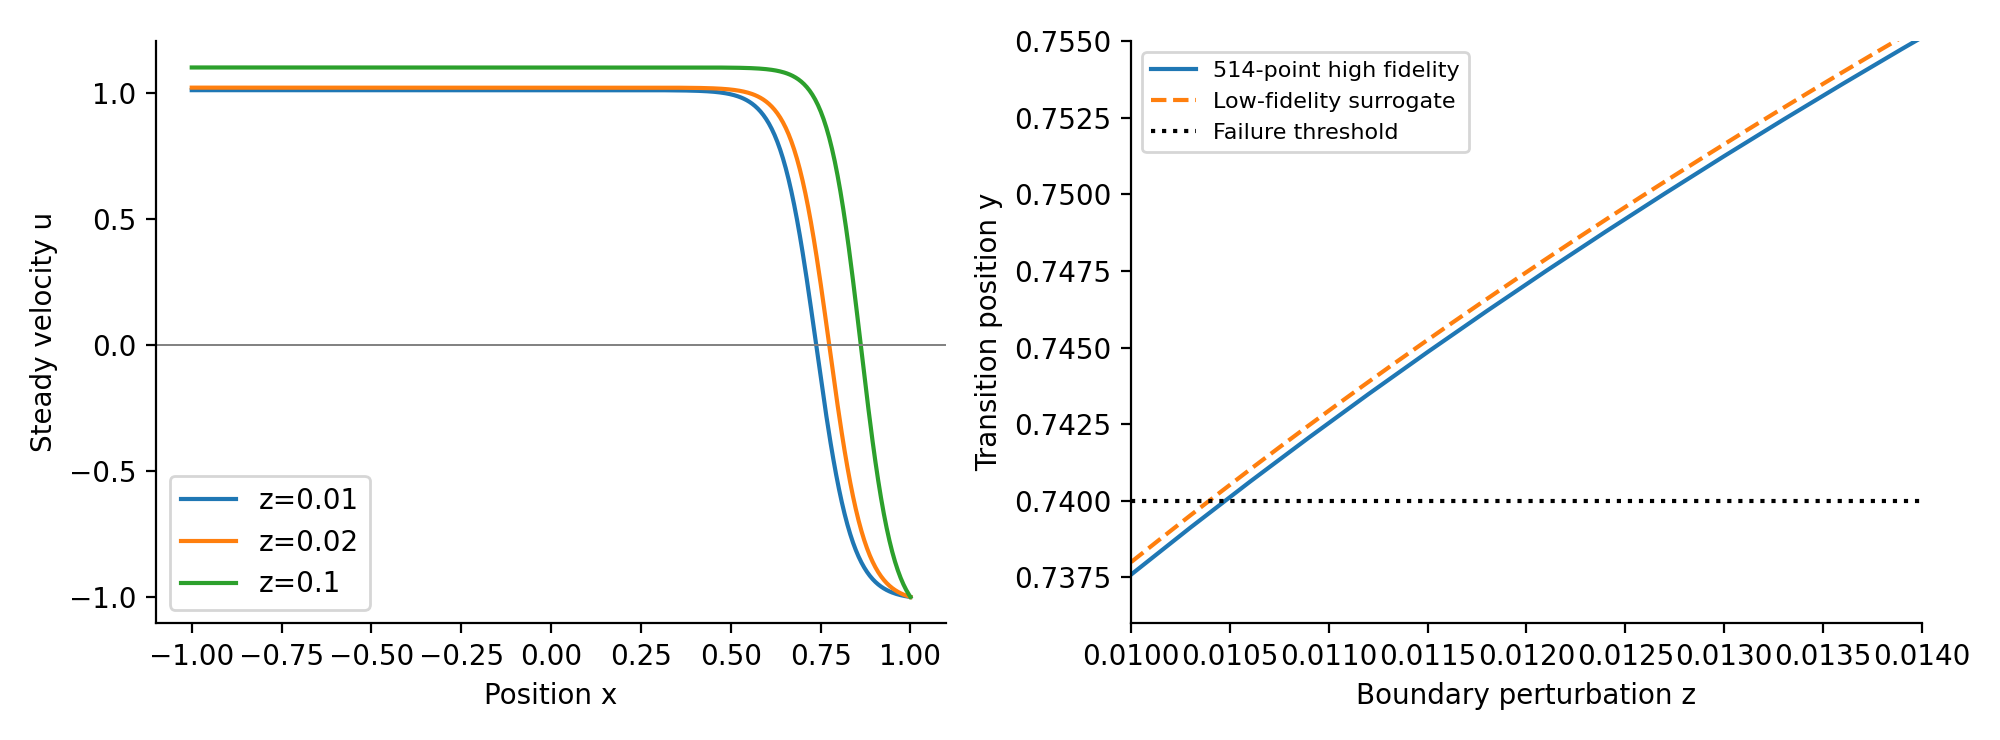
\includegraphics[width=\linewidth]{figures/burgers.png}
\caption{Left, each curve crosses zero where the steady flow changes direction. Right, points below the dotted line correspond to a change of direction before the mark at 0.74. The dashed curve shows the interpolated surrogate used in the simulations.}\label{fig:burgers}
\end{figure}

To read Figure~\ref{fig:burgers}, first choose one value of $z$. In the left panel, follow its velocity curve to $u=0$ and read off the horizontal coordinate $x$. That coordinate is the output $y$ for this simulation. Now compare the blue and green curves. When $z$ increases, the rightward flow at the left end is stronger. The green curve stays positive farther along the channel, so the change of direction moves to the right. In the right panel, each input $z$ is now paired with its output $y$. For example, the fine-grid calculation gives $y=0.73913$ at $z=0.0103$ (failure) and $y=0.74062$ at $z=0.0106$ (safe). Here being \emph{below} the threshold counts as failure. The indicator therefore equals one for the first input and zero for the second.

The paper reads the transition position at the final time of its numerical integration on 514 grid points and builds a surrogate using proper orthogonal decomposition (POD), which approximates the velocity profile using 20 patterns extracted from earlier simulations. The paper used one million draws to construct its Burgers sampling density. Here we use 20,000. The boundary conditions, viscosity and failure threshold are the same. To simplify the calculation, the high-fidelity model solves directly for the steady flow on 514 points. The surrogate uses a coarser grid of 258 points at 81 values of $z$ and interpolates between those results. The 258 points describe positions along the flow for one simulation. The 81 values of $z$ describe different boundary conditions, each requiring a separate coarse simulation. After those 81 solves, the position for a new pilot input is estimated from nearby stored results. The final MFIS check still solves on the fine grid at the newly drawn input.

On the 514-point grid, $y$ reaches 0.74 at $z\approx0.0104744$. Values of $z$ below this boundary give failure. Because $z$ is uniform, the reference probability is the width of the failure interval divided by the width of the full input range:
\begin{equation}
P_{\mathrm{ref}}=\frac{0.0104744-0.01}{0.1-0.01}\approx0.005271.
\end{equation}
The paper reports a Monte Carlo estimate of 0.00549 from one million draws, with an estimated RMSE of about 0.000074. Our grid gives 0.005498 at 1,026 points and 0.005555 at 2,050 points. The closeness at 1,026 points alone cannot establish that the two implementations agree. This illustrates two different errors. Changing the grid changes the probability predicted by the flow model. Taking more random samples on a fixed grid only reduces the error in estimating that grid's probability.

\begin{table}[H]\centering\small
\begin{tabular}{lrrrr}
\toprule
Method & Mean estimate & RMSE & Rel. RMSE & Coverage \\
\midrule
MC & 0.005450 & 1.65e-03 & 31.3\% & 97.5\% \\
HF IS & 0.005272 & 7.14e-05 & 1.4\% & 97.5\% \\
MFIS & 0.005291 & 1.25e-04 & 2.4\% & 100.0\% \\
Surrogate IS & 0.004378 & 8.95e-04 & 17.0\% & 0.0\% \\
\bottomrule
\end{tabular}
\caption{Burgers results at $n=2{,}000$ with 40 runs. Errors and normal-interval coverage refer to the 514-point numerical model. Pilot and surrogate-construction costs are separate.}\label{tab:burgers}
\end{table}

MFIS reduced the relative RMSE from 31.3\% for MC to 2.4\%. The surrogate predicted a failure probability of about 0.00438, below the reference of 0.00527. For instance, at $z=0.01043$ the fine grid gives a failure and the surrogate gives a safe result. This explains why surrogate IS still had a 17.0\% relative RMSE: it kept checking failure against the same shifted boundary. MFIS used that surrogate to find the neighbourhood of the boundary, then checked each in-range final draw on the finer grid.

HF IS had the smallest error, but its pilot took about 1.61 seconds. For MFIS, building the interpolant took about 0.008 seconds and running the pilot took about 0.001 seconds. Both methods still used the fine grid for production draws inside the input range. These times compare setup costs on one computer.

\section{New example: stopping distance of a sliding block}
\subsection{What happens after the push?}
Imagine pushing a wooden block across a rough, level floor and letting go. Start measuring at the instant you let go. The block is already moving. Friction slows it until it stops. Draw a chalk line 24.01 m ahead of the release point. A gentle push leaves the block short of the line. A hard enough push sends it past the line before it stops. We call passing the line a failure. This gives us a yes-or-no outcome for each push.

Now repeat the experiment from the same spot with the same block and floor. Only the speed at release changes. We assume this speed $v$ is uniform between 0 and 10 m/s, so a speed between 8 and 9 m/s is as likely as one between 9 and 10 m/s. What fraction of all these releases carry the block past the chalk line?

\subsection{How fast must the block start?}
At release, a block of mass $m$ has kinetic energy $mv^2/2$. As it slides, friction removes this energy. The floor supports the block's weight $mg$, so the magnitude of kinetic friction is $\mu_k mg$, where $\mu_k=0.20$ is the fixed coefficient of kinetic friction. This force is constant, so each metre of sliding removes the same amount of energy. By the time the block has slid a distance $d_H$ and stopped, friction has removed all its initial kinetic energy. This gives
\begin{equation}
\mu_k mg\,d_H=\tfrac12 mv^2,\qquad d_H(v)=\frac{v^2}{2\mu_k g}=\frac{v^2}{4},
\end{equation}
where $g=10$ m/s$^2$ and the distance is in metres when $v$ is in m/s. Doubling the release speed gives the block four times the energy, so it slides four times as far.

At 8 m/s the block slides $8^2/4=16$ m and stops short. At 10 m/s it slides 25 m and passes the line. To find the speed between these outcomes, set the stopping distance equal to 24.01 m. This gives $v=\sqrt{4(24.01)}=9.8$ m/s. At exactly this speed the block stops on the line. The code compares release speeds with this cutoff to decide crossings. Faster releases pass it. The crossing speeds therefore occupy only the last 0.2 m/s of a 10 m/s range. Since speed is uniform, the probability is
\[
P(\text{block passes the line})=\frac{10-9.8}{10-0}=0.02.
\]
Over many ordinary releases we would expect about two crossings per hundred. We can use this exact result to check what the sampling methods give us.

\subsection{Making a simpler model of the same block}
The energy formula is the high-fidelity model in this example: it defines which outcomes count as failures. To see what happens when we use a less accurate model, we deliberately approximate its curve with a straight line. This is the low-fidelity model, also called a surrogate. For the surrogate, take the tangent to the distance curve at 9 m/s. The distance there is 20.25 m and the slope is $9/2=4.5$, since differentiating $v^2/4$ gives $v/2$, so
\begin{equation}
d_L(v)=20.25+4.5(v-9).
\end{equation}
The left panel of Figure~\ref{fig:block} compares the two predictions. Each point on a curve gives the final stopping distance for one release speed. The horizontal dotted line is the distance to the chalk mark. Consider a starting speed of 9.82 m/s. The energy calculation gives 24.1081 m, just past the line. The tangent gives 23.94 m, just short of it. The surrogate only predicts a crossing above about 9.8356 m/s, so it misses a small interval of speeds. To obtain its cutoff, set $20.25+4.5(v-9)=24.01$ and solve for $v$. Far below 9 m/s the tangent can even give a negative distance. We use it only to flag possible crossings. The fraction of the input interval above this new cutoff is $(10-9.8356)/10\approx0.01644$. At 9.82 m/s, for example, MFIS would count a weighted crossing and surrogate IS would record zero. Counting only the crossings predicted by the tangent would therefore underestimate the probability, even with a very large sample.

\subsection{Counting crossings with ordinary Monte Carlo}
Suppose we knew how to evaluate the distance at each speed but did not know how to solve for the cutoff. We could draw speeds uniformly, calculate the distance each time, and count crossings. Write 1 for a crossing and 0 for a stop before or exactly on the line. For instance, speeds of 8, 9.82 and 9 m/s give distances of 16, 24.1081 and 20.25 m. Their three entries are 0, 1 and 0. Adding the entries counts crossings, and dividing by the number of draws gives their fraction. These three speeds illustrate the arithmetic.

In the first actual MC run with 2,000 speeds, 31 crossed. The estimate was $31/2000=0.0155$. With a true probability of 0.02 we expect 40 crossings on average, but the number varies each time we draw a fresh set. This variation is sampling error. For the block another 2,000 distance calculations are cheap. For a flow simulation the same number of calculations can be expensive.

\subsection{Following one run from pilot to estimate}
To observe more crossings, we can deliberately test more fast releases. First we need to locate those speeds. For this preliminary step, called the pilot, we drew 20,000 uniform speeds. The tangent flagged 360 of them as crossings. We kept those 360 \emph{speeds}: their mean, 9.923 m/s, locates the centre of the Gaussian and their standard deviation, 0.047 m/s, sets its width. The pilot fraction $360/20{,}000$ describes what the tangent predicted in that sample. The purpose of the pilot here is to learn where to draw the next set of speeds.
\begin{figure}[H]\centering
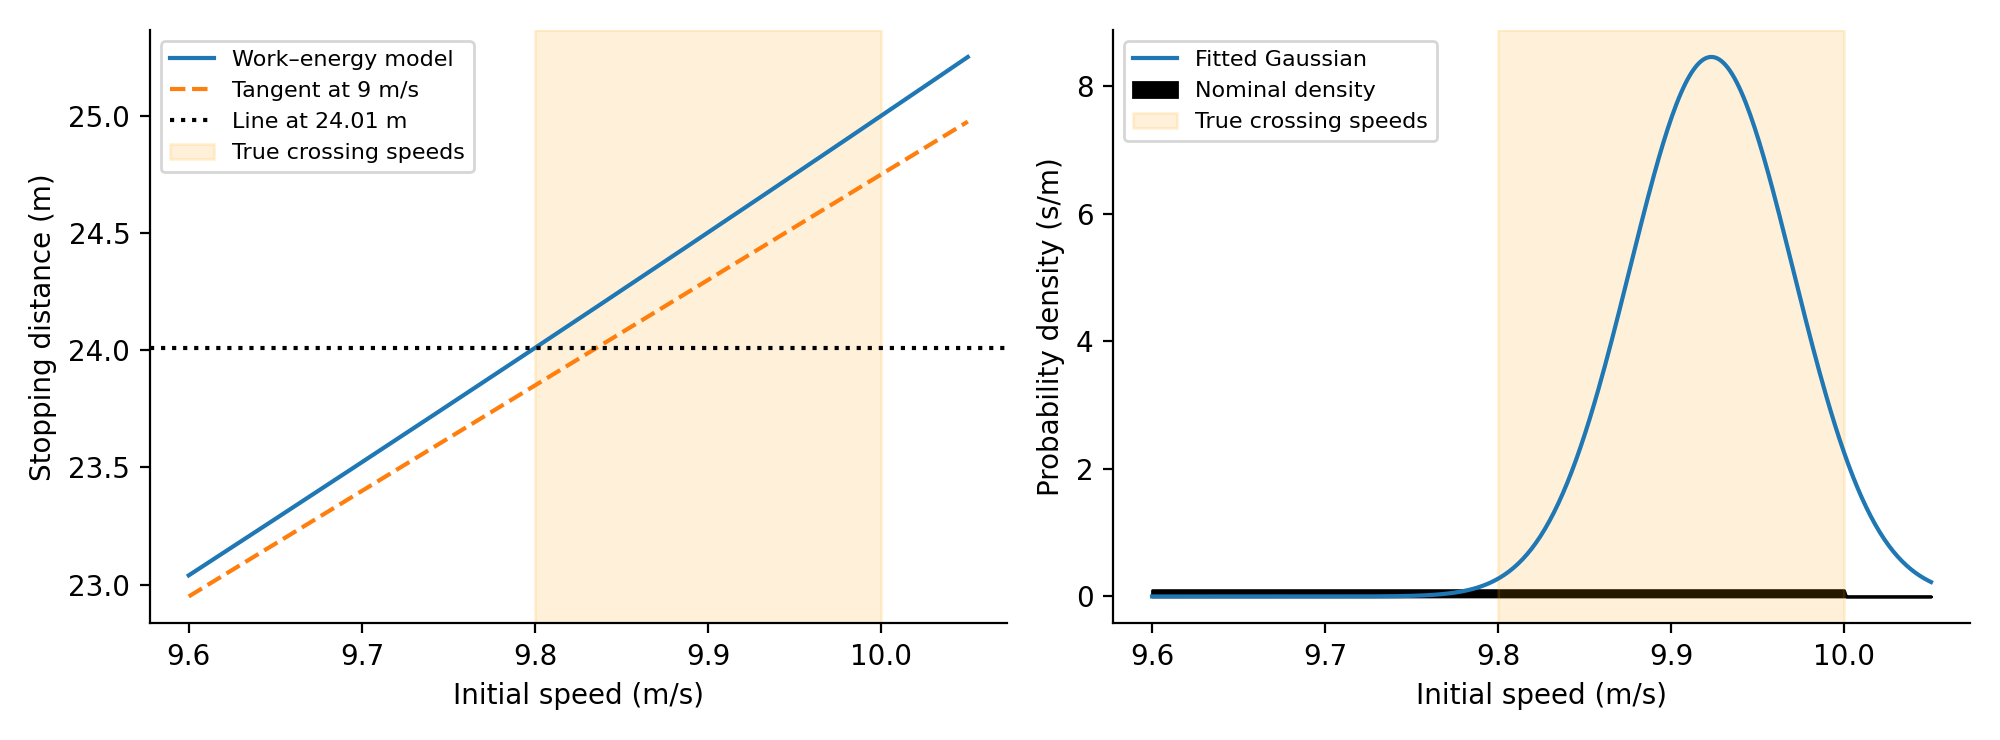
\includegraphics[width=\linewidth]{figures/sliding_block.png}
\caption{Stopping distance near the line and the proposal fitted from surrogate crossings.}\label{fig:block}
\end{figure}


The right panel of Figure~\ref{fig:block} shows how we choose the fresh speeds. The flat black density represents ordinary releases. The blue curve concentrates test speeds near the shaded crossing region. The motion of the block at any given speed stays the same. What changes is how often we test that speed range.

In the first MFIS run with 2,000 fresh draws, 1,906 were inside the allowed range and crossed the line. The raw fraction would be $1906/2000=95.3\%$. This answers a different question: how often does a crossing occur when we deliberately choose speeds near 9.923 m/s? The question about the original uniform speeds still has the answer 2\%.

Consider the first draw, $v=9.93335$ m/s. Under the original uniform distribution, $\rho(v)=1/10=0.1$ per m/s. At this speed the fitted Gaussian density is $q(v)\approx8.262$ per m/s. These are densities: for a very narrow interval around that speed, its probability is approximately its density times its width. The Gaussian therefore samples this neighbourhood about $8.262/0.1=82.62$ times as often. To compensate, this crossing contributes $1/82.62\approx0.01210$ to the sum.

Two other draws show why zeros matter. Draw 93 was 9.77467 m/s. It was inside the original range but the block stopped short, so its indicator was zero. Draw 29 was 10.01886 m/s. The Gaussian can generate it, but the original model gives speeds above 10 zero density. Its contribution was also zero. Both draws count towards the 2,000 used in the denominator.

Adding all 2,000 weighted contributions gave 39.57176. Dividing by 2,000 gave $0.019786$, or about 1.98\%. The original MC run counted 31 crossings with weight one. This MFIS run observed many more crossings, each with a weight determined by its speed. Both calculations estimate the same probability.

\subsection{Reading the sliding-block results}
\begin{table}[H]\centering\small
\begin{tabular}{lrrrr}
\toprule
Method & Mean estimate & RMSE & Rel. RMSE & Coverage \\
\midrule
MC & 0.019775 & 2.99e-03 & 14.9\% & 100.0\% \\
HF IS & 0.019984 & 1.74e-04 & 0.9\% & 97.5\% \\
MFIS & 0.019932 & 5.22e-04 & 2.6\% & 90.0\% \\
Surrogate IS & 0.016484 & 3.52e-03 & 17.6\% & 0.0\% \\
\bottomrule
\end{tabular}
\caption{Sliding-block estimates over 40 runs of 2,000 production draws each. The exact reference probability is 0.02.}\label{tab:block}
\end{table}

The mean MFIS estimate was 0.019932, close to the exact probability of 0.02. Its relative RMSE was 2.6\%, compared with 14.9\% for ordinary MC. Surrogate IS gave 0.016484 on average, close to the value predicted by the tangent. Both distance formulas are cheap to evaluate. The point of this example is that we can check the method by hand.


For example, the first MFIS run has error $0.019786-0.020000=-0.000214$. Other runs can err in the opposite direction. Squaring each error before averaging prevents them from cancelling. Across the 40 MFIS runs the RMSE was about 0.000522, or $100(0.000522/0.02)=2.61\%$ of the reference probability. This explains how the 2.6\% entry can appear alongside a mean estimate of 0.019932. One number measures the size of individual run errors; the other averages the estimates themselves. In the same row, 90\% coverage means that 36 of the 40 intervals contained 0.02. Each interval accounts for 2.5 percentage points of coverage, so 40 runs give limited precision for judging the interval method.

\section{Conclusion}
In the block example the surrogate misses real crossings just above 9.8 m/s, but it still points to the right end of the speed range. Checking fresh draws with the energy model and weighting them by $\rho/q$ gives the desired probability on average. In Table~\ref{tab:block}, the mean estimate rises from 0.016484 for surrogate IS to 0.019932 for MFIS. Both draw from the same fitted density. The difference is which model is allowed to decide that a crossing occurred. The Burgers example adds a practical reason for using a surrogate: searching for likely failures by interpolation costs much less than solving the flow equations for every pilot input.

At 2,000 production draws, MFIS reduced relative RMSE from 31.3\% to 2.4\% for the flow and from 14.9\% to 2.6\% for the block. These figures compare the accuracy of the estimates for the fitted proposals. MC needs no pilot, so equal production counts do not establish equal total computing cost. Both problems have one uncertain input and one failure interval. If the surrogate missed a separate failure region, the fitted proposal could sample it very rarely. This limits what we can conclude from these two examples.

\section*{Code and reproducibility}
GitHub repository for the Python code, run instructions and saved results:
\url{https://github.com/dohuyenanh/Multi-fidelity-importance-sampling.git}.

AI assistance was used to develop the implementation and revise the wording of the report.
\end{document}
